\frame{\tableofcontents}

%---------------------------------------------------------------------------
\begin{frame}
\frametitle{Un poco de historia...}

\begin{columns}
\begin{column}{0.5\textwidth}
	\begin{itemize}
		\item{Teor\'ia BCS $\longrightarrow$ Existe un gap de energ\'ia}
		\item{Medidas indirectas}
		\item{Giaever lo consigue medir directamente}
		\item{Premio Nobel en 1973}
	\end{itemize}
\end{column}
\begin{column}{0.5\textwidth}
	\begin{figure}[!h] \label{giaever60}
	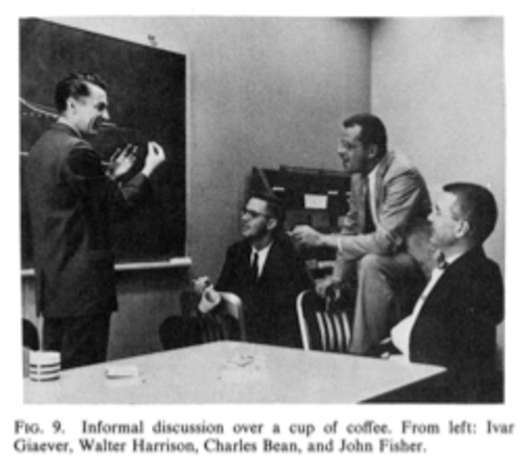
\includegraphics[width=0.6\textwidth]{giaever60}
	\end{figure}
	\begin{figure}[!h] \label{giaever99}
	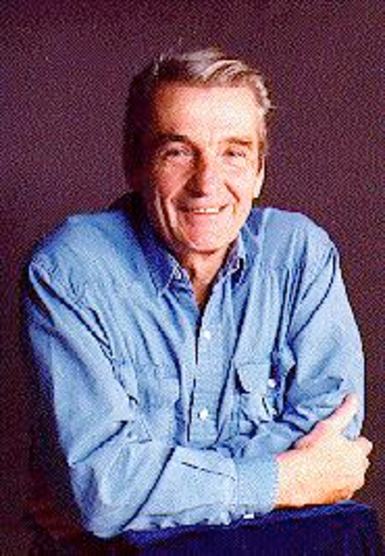
\includegraphics[width=0.4\textwidth]{giaever99}
	\end{figure}
\end{column}
\end{columns}

\end{frame}
 %---------------------------------------------------------------------------  
%---------------------------------------------------------------------------
\begin{frame}
\frametitle{Objetivos}

\begin{itemize}
	\item{Produce Samples}
	\item{Measure Current}
	\item{Calculate Gap}
\end{itemize}

\end{frame}
%---------------------------------------------------------------------------